\chapter{Onde ed Equazione di Schr\"odinger}

\begin{definition}
Definiamo \textbf{acca tagliato} come
\[\hbar=\frac h{2\pi}.\]
\end{definition}

\noindent
Per semplicit\`a faremo quantistica in una sola dimensione.

\section{Richiami di onde}
\begin{definition}[Onda]
Un'\textbf{onda} \`e una funzione di posizione e tempo della forma
\[f(x,y)=f(kx-\omega t).\]
La \textbf{lunghezza d'onda} \`e $\la=\frac{2\pi}k$ e la sua \textbf{frequenza} \`e $\nu=\frac\omega{2\pi}$.\\
La velocit\`a di un'onda o \textbf{velocit\`a di fase} \`e $\frac{\omega}k=\nu\la$.
\end{definition}

\noindent
Se l'onda si comporta anche come una particella, la velocit\`a di questa particella \`e la velocit\`a di fase?
\begin{itemize}
\item Caso non relativistico:
\[\begin{cases}
p=mv\\
E=\frac12mv^2
\end{cases}\implies v_{\text{particella}}=\frac{2E}p=\frac{2h\nu}{h/\la}=2\nu\la\neq \nu\la.\]
\item Caso relativistico:
\[\begin{cases}
p=mv\gamma\\
E=mc^2\gamma
\end{cases}\implies v_{\text{particella}}=\frac{pc^2}E=\frac{hc^2}{h\la\nu}=\frac{c^2}{\la\nu}\]
e questa quantit\`a vale $\la\nu$ solo se $\la\nu=c$, ma non tutte le particelle che vogliamo trattare vanno alla velocit\`a della luce.
\end{itemize}
\noindent La giusta definizione di $v_{\text{particella}}$ \`e

\begin{definition}[Velocit\`a di gruppo]
La \textbf{velocit\`a di gruppo} di un'onda \`e
\[v_{\text{particella}}=\dd k\omega.\]
\end{definition}

\noindent
Se l'onda in esame \`e una semplice sinusoide allora le due velocit\`a coincidono, ma se consideriamo somme di diverse sinusoidi\footnote{per esempio in una serie di Fourier} allora le due quantit\`a sono distinte e $v_{\text{particella}}$ \`e la misura di velocit\`a giusta per l'insieme delle onde.

\begin{remark}
Dato che $E=h\nu$ e $\la=h/p\coimplies p=\frac h{2\pi}k$ si ha che $E=\hbar\omega$ e $\vec p=\hbar \vec k$. In effetti
\[(2\pi\nu/c,\vec k)\]
\`e un quadrivettore.
\end{remark}


\section{Esperimento della doppia fenditura}
Consideriamo due pareti parallele, di cui la pi\`u vicina con due fessure. Due versioni standard di questo esperimento sono

\begin{itemize}
\item Se lanciamo delle palline al primo muro, quelle che passano vengono rilevate dal secondo muro e viene tenuto conto di dove le palline colpiscono la parete. 

\begin{figure}[!htb]
    \centering
    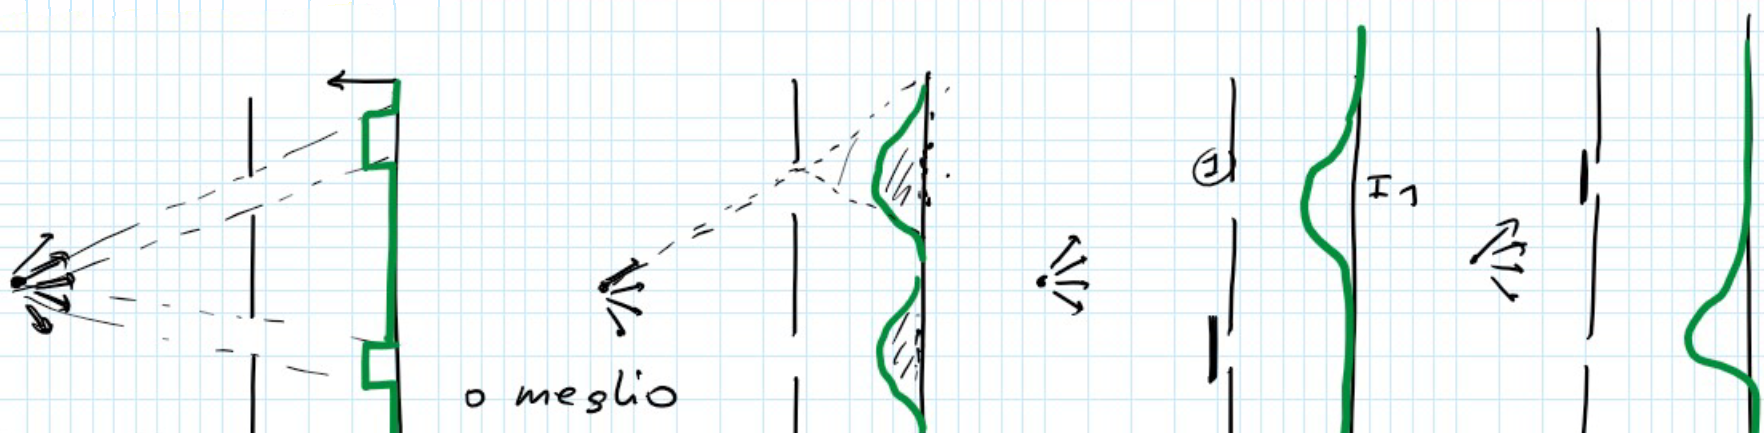
\includegraphics[width=11cm]{images/Double_slit_palline.png}
\end{figure}

\item Consideriamo ora una sorgente puntiforme prima del primo muro. Se chiudiamo una fenditura non succede niente di inaspettato, ma aprendole entrambe troviamo un pattern di interferenza.

\begin{figure}[!htb]
    \centering
    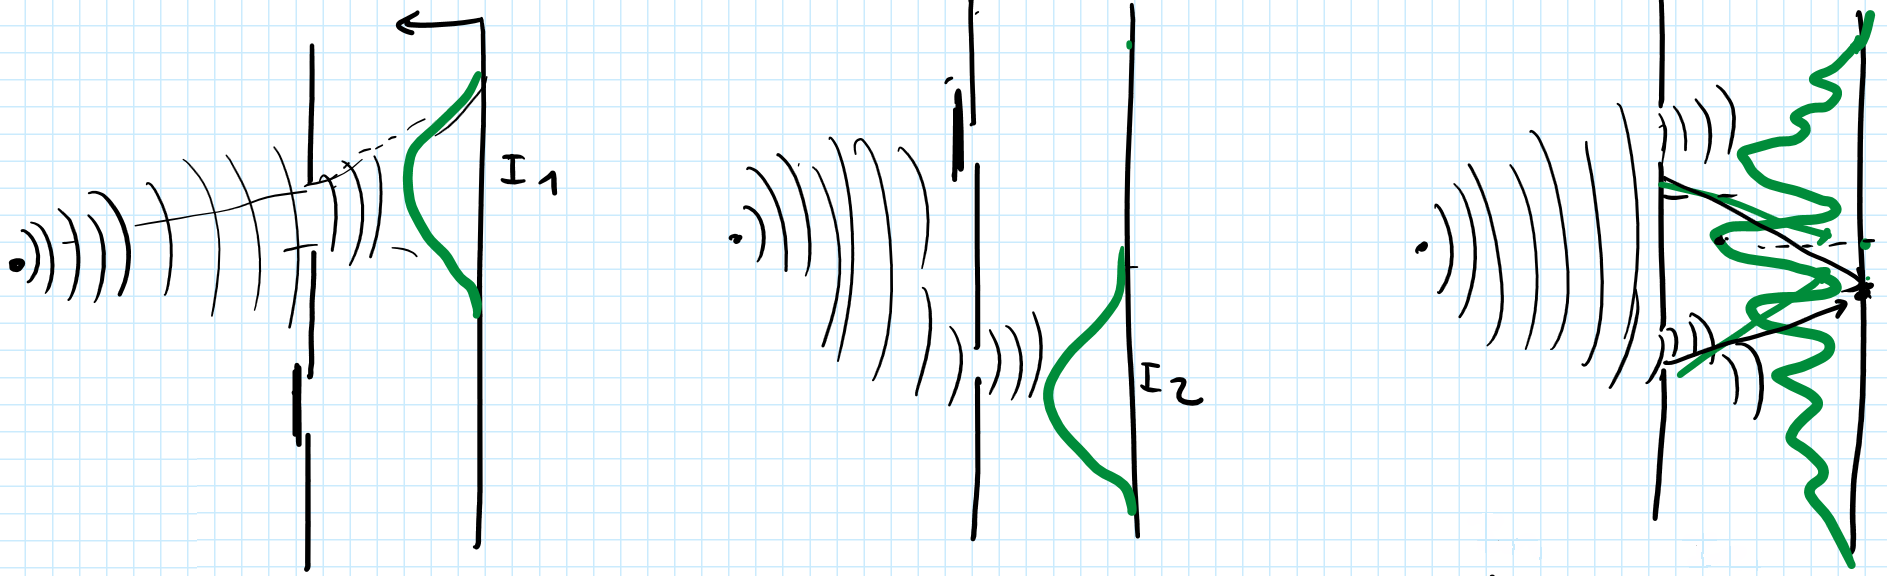
\includegraphics[width=11cm]{images/double_slit_onda.png}
\end{figure}
\end{itemize}

\newpage
\noindent
Come si comporta un elettrone se facciamo questo esperimento? Se lanciamo tanti elettroni uno alla volta troviamo lo stesso pattern di interferenza delle onde.

\begin{figure}[!htb]
    \centering
    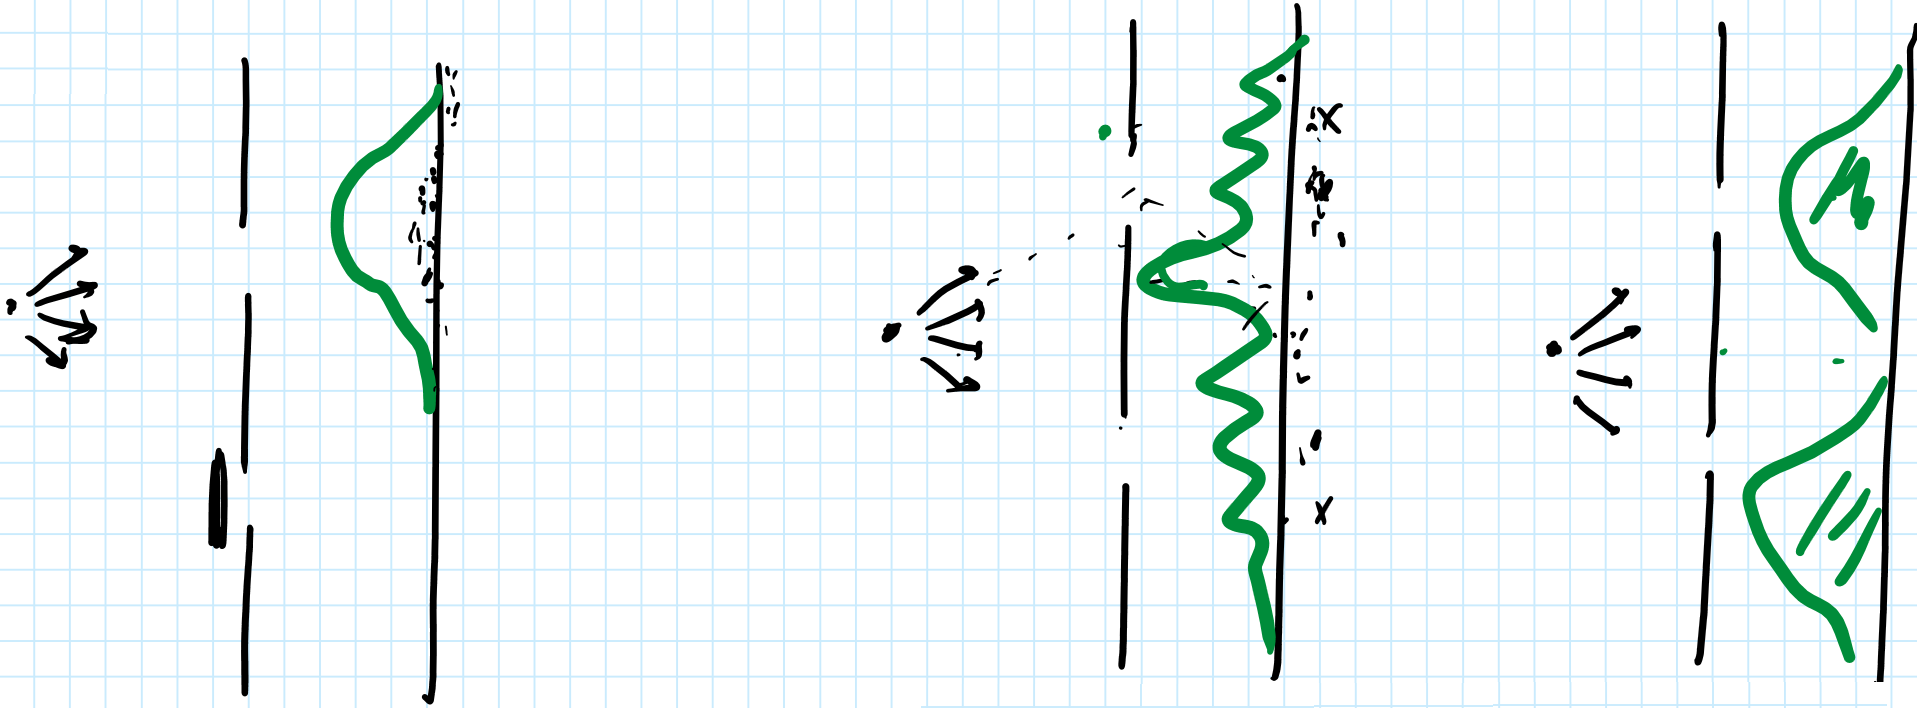
\includegraphics[width=11cm]{images/double_slit_elettroni.png}
\end{figure}

\bigskip

\noindent
Supponiamo ora di inserire dei rilevatori sulle fenditure che ci informano su quale fessura riceve qualche elettrone.
Scopriamo che se mandiamo un elettrone alla volta i rilevatori non si attivano mai contemporaneamente e il pattern in arrivo cambia e torna simile al caso delle palline.\bigskip


Possiamo ipotizzare che il rilevatore sia troppo pesante, fino al punto da modificare l'elettrone a sufficienza da cambiare l'esito.\\
Proviamo a usare una luce molto fioca. Quando rileviamo un elettrone ci segnamo da quale fenditura \`e passato o se non lo abbiamo rilevato (magari la luce \`e cos\`i fioca che a volte non rileva l'elettrone).\\
Il risultato \`e che se l'elettrone \`e stato rilevato si comporta come una pallina, altrimenti segue il pattern di interferenza.
\begin{figure}[!htb]
    \centering
    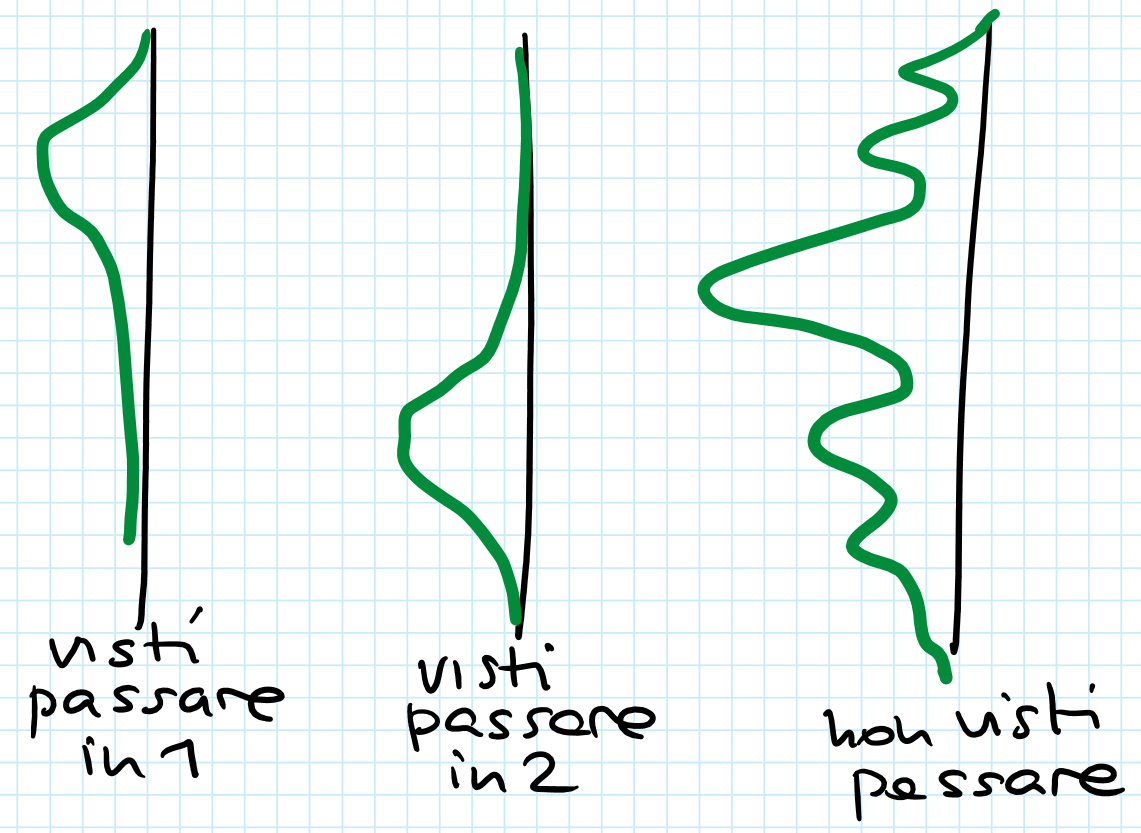
\includegraphics[width=6cm]{images/visti_passare_o_non_visti.png}
\end{figure}


Anche diminuendo la frequenza riscontriamo lo stesso fenomeno finch\'e la lunghezza d'onda non supera la distanza tra le fessure, da quel punto l'elettrone segue sempre il pattern di interferenza.\bigskip


In in qualche modo c'\`e una ``interazione minima" che l'elettrone pu\`o subire. Se avviene una interazione che ci permette di rilevare quale fessura \`e stata attraversata allora l'energia neccessaria \`e stata tale da modificare l'elettrone, se invece usiamo frequenze abbastanza basse, in modo da scendere sotto la soglia di energia di interazione minima, allora l'elettrone pu\`o restare inalterato e comportarsi come un'onda, ma non riusciamo a capire attraverso quale fessura \`e passato.

\subsection{Interpretazione}
\begin{fact}[Interpretazione di Copenhagen]
\textbf{Prima di una misura, la posizione di una particella non \`e ben definita.}
\end{fact}

\begin{theorem}[Bell]
Esistono degli esperimenti che ci permetterebbero di verificare se la quantistica \`e completa o se potrebbero esistere ``variabili nascoste". 
\end{theorem}
\begin{fact}
Facendo gli esperimenti descritti da Bell la meccanica quantistica \`e verificata.
\end{fact}


\noindent
Ma quindi la materia in generale di comporta come un'onda? Si ma a livelli macroscopici non si nota. 

\begin{remark}
Per un fotone abbiamo
\[h\frac c\la=h\nu=E\pasgnl={luce}pc\implies \la=\frac hp.\]
\end{remark}

\noindent
De Broglie usa la stessa formula per la lunghezza d'onda caratteristica di un oggetto:
\[\la=\frac hp,\]
dove $p$ \`e la quantit\`a di moto.\\
Per un oggetto macroscopico $\la$ \`e molto piccolo, in particolare molto pi\`u piccolo delle dimensioni dell'oggetto, rendendo effetti quantistici impercettibili.\\
Per esempio, effetti di diffrazione si verificano quando la fenditura ha una larghezza simile alla lunghezza d'onda.



\section{Equazione di Schr\"odinger}

\begin{theorem}[Equazione di Schr\"odinger]\label{EquazioneSchrodinger}
Per onde vale l'\textbf{equazione di Schr\"odinger}
\[\boxed{i\hbar \pp t\psi=-\frac{\hbar^2}{2m}\pps[2]x\psi +V(x)\psi}\]
dove $V$ \`e un termine di energia potenziale.
\end{theorem}
\begin{proof}[Derivazione intuitiva]
Trascuriamo momentaneamente la relativit\`a.
\[E=\frac12mv^2+V(x)=\frac{p^2}{2m}+V(x).\]
Poich\'e $E=\hbar \omega$ e $p=\hbar k$ si ha che
\[\hbar \omega=\frac{\hbar^2}{2m}k^2+V.\]
Sia $\psi(x,t)$ l'equazione dell'onda. In particolare consideriamo
\[\psi(x,t)=Ae^{i(kx-\omega t)}.\]
Notiamo che
\[\pp t\psi=-i\omega\psi,\quad \pp x\psi=ik\psi,\quad \pps[2]x\psi=-k^2\psi,\]
dunque mettendo tutto insieme
\[i\hbar \pp t\psi=-\frac{\hbar^2}{2m}\pps[2]x\psi +V(x)\psi.\]
\end{proof}
\begin{center}
``Ma i numeri complessi che ci fanno in fisica?''
\end{center}
L'interpretazione fisica di $\psi$ \`e che $\abs{\psi(x,t)}^2\geq 0$ rappresenta la \textit{densit\`a di probabilit\`a di trovare la particella nel punto $x$ al tempo $t$}.
\bigskip

\noindent
Abbiamo quindi rinunciato a trovare una posizione esatta. Sappiamo solo delle probabilit\`a.


\begin{remark}
$\abs{\psi(x,t)}^2$ \`e la \textit{densit\`a di probabilit\`a} di trovare la particella in $x$ al tempo $t$, cio\`e $\abs{\psi(x,y)}^2dx$ \`e la probabilit\`a di trovare la particella tra $x$ e $x+dx$.
\end{remark}

\noindent Affinch\'e questo modulo rappresenti una densit\`a di probabilit\`a vogliamo
\[\int_{-\infty}^\infty\abs{\psi(x,t)}^2dx=1.\]
Poich\'e abbiamo integrato solo lungo $x$, a priori questo integrale dipende da $t$, ma\footnote{per questo conto supponiamo $V(x)=0$. Abbiamo anche usato il fatto che $\psi^\ast$ rispetta l'equazione coniugata $-i\hbar \pp t{\psi^\ast}=-\frac{\hbar^2}{2m}\pps[2]x{\psi^\ast} +V(x){\psi^\ast}$}
\begin{align*}
\dd t{}\int_{-\infty}^\infty \abs{\psi(x,t)}^2dx=&\int_{-\infty}^\infty \pp t{}\abs{\psi(x,t)}^2dx=\\
=&\int_{-\infty}^\infty\pa{\pp t{\psi^\ast}\psi+\psi^\ast\pp t{\psi}}dx=\\
=&\frac{i\hbar}{2m}\int_{-\infty}^\infty \pa{\psi^\ast\pps[2]x\psi-\pps[2]x{\psi^\ast}\psi}dx=\\
=&\frac{i\hbar}{2m}\int_{-\infty}^\infty \pp x{}\pa{\psi^\ast\pp x\psi-\pp x{\psi^\ast}\psi}dx=\\
=&\frac{i\hbar}{2m}\spa{\psi^\ast\pp x\psi-\pp x{\psi^\ast}\psi}^\infty_{-\infty}=0.
\end{align*}
Stiamo assumendo che $\abs{\psi(x,t)}^2$ sia dominata da una funzione integrabile, ma se vogliamo sperare in soluzioni fisicamente rilevanti questo \`e certamente ragionevole.

\section{Equazione a variabili separabili}
In questa sezione supponiamo $\psi(x,t)=g(t)f(x)$. Sostituendo nell'equazione di Schr\"odinger troviamo
\[i\hbar g'f=-\frac{\hbar^2}{2m}gf''+V(x)gf,\]
da cui
\[i\hbar \frac{g'}g=-\frac{\hbar^2}{2m}\frac{f''}f+V(x).\]
Ricordando da dove \`e venuta fuori l'equazione di Schrodinger, questa ultima equazione corrisponde all'energia dell'onda $E$, dunque
\[\begin{cases}
~\\
\displaystyle i\hbar \dd tg=Eg\\\\
\displaystyle-\frac{\hbar^2}{2m}\dds[2]xf+V(x)f=Ef\\~
\end{cases}\]
La prima equazione ha soluzioni del tipo $g(t)=Ce^{-Et/\hbar}=Ce^{-i\omega t}$. 

\begin{definition}[Equazione di Schr\"odinger indipendente dal tempo]
L'\textbf{equazione di Schr\"odinger indipendente dal tempo} \`e
\[-\frac{\hbar^2}{2m}\dds[2]xf+V(x)f=Ef.\]
\end{definition}
\begin{remark}
L'equazione di Sch\"odinger indipendente dal tempo \`e una equazione differenziale che non coinvolge numeri complessi, quindi le sue soluzioni sono reali a meno di un termine di fase.
\end{remark}



\begin{definition}[Soluzioni stazionarie]
Una soluzione dell'equazione di Sch\"odinger \`e \textbf{stazionaria} se $\abs{\psi(x,t)}^2$ non dipende dal tempo.
\end{definition}

\begin{remark}
Nell'ipotesi di variabili separabili, le soluzioni sono stazionarie, infatti
\[\psi(x,t)=Ce^{-i\omega t}f(x)\implies \abs{\psi(x,t)}^2=\abs{C}^2f^2(x).\] 
\end{remark}


\begin{remark}
Se $f_1,\ f_2$ ecc sono soluzioni per l'equazione di Sch\"odinger indipendente dal tempo con energie $E_1, E_2$ ecc, allora funzioni della seguente forme sono soluzioni dell'equazione di Schr\"odinger
\[\psi(x,t)=a_1e^{-iE_1 t/\hbar}f_1(x)+a_2e^{-iE_2 t/\hbar}f_2(x)+\cdots\]
In particolare per risultati di analisi possiamo scrivere ogni soluzione come combinazione lineare di soluzioni stazionarie.
\end{remark}




\begin{remark}
Se $f$ \`e una soluzione dell'equazione di Schr\"odinger indipendente dal tempo tale che $\lim_{\abs{x}\to\infty} f(x)=0$, allora
\begin{itemize}
\item $f$ \`e non degenere (le altre soluzioni solo solo versioni riscalate)
\item $f$ \`e reale a meno di un termine di fase.
\end{itemize}
\end{remark}
\begin{proof}
Supponiamo che ci siano due soluzioni $f$ e $\wt f$, allora
\[\frac{\wt f''}{\wt f}=\frac{f''}f=-\frac{2m}{\hbar^2}(E-V),\]
quindi
\[0=\wt f'' f-f''\wt f=\dd x{}\pa{\wt f' f-f'\wt f},\]
cio\`e $\wt f' f-f'\wt f$ \`e costante, ma dato che $f\to 0$ per $\abs{x}\to\infty$ si ha che l'unica costante possibile \`e $0$. Quindi
\[\wt f'f=f'\wt f\implies \log \wt f=\log f + cost.\implies \wt f=cf.\]
Inoltre, poich\'e l'equazione ha coefficienti reali, se $f$ \`e soluzione anche $f^\ast$ lo \`e, dunque $f^\ast=cf$.
\[f=c^\ast f^\ast\implies cf=f^\ast=\frac f{c^\ast}\implies \abs{c}^2=1,\]
cio\`e $c=e^{i\theta}$ per qualche fase $\theta$. Se $f=r(x)e^{i\al(x)}$ allora $f^\ast=r(x)e^{-i\al(x)}$, quindi questo risultato mostra $\al(x)+\theta=-\al(x)$, cio\`e $\al(x)=-\theta/2$ \`e costante in $x$, cio\`e $f$ \`e una funzione reale a meno di una fase.
\end{proof}


\subsection{Esempi di soluzioni al variare del potenziale}
\subsubsection{Potenziale costante}
Consideriamo un potensiale del tipo
\[V(x)=V_0\]
e studiamo solo onde standard $\psi=Ae^{-i(\omega t-kx)}=e^{-i\omega t}f(x)$. Dall'equazione di Schr\"odinger indipendente dal tempo troviamo
\[E=\frac{\hbar^2 k^2}{2m}+V_0\implies k=\pm\sqrt{\frac{2m(E-V_0)}{\hbar^2}}.\]
Consideriamo il problema al variare del segno di $E-V_0$:
\setlength{\leftmargini}{0cm}
\begin{itemize}
\item[$\boxed{E>V_0}$] In questo caso 
\[\psi(x,t)=Ae^{-i(\omega t-kx)}+Be^{-i(\omega t+kx)}\]
ma queste soluzioni \underline{non sono normalizzabili}, per esempio se $B=0$ allora $\abs{\psi}^2=A$ e quindi l'integrale diverge se $A\neq 0$.
\item[$\boxed{E<V_0}$] (In questo caso non ci aspettiamo soluzioni.)\\
In questo caso i valori di $k$ sono immaginari puri quindi poniamo $k=i\al$.
\[\psi(x,t)=e^{-i\omega t}\pa{Ae^{\al x}+B e^{-\al x}}.\]
Affinch\'e ci sia convergenza sia a $+\infty$ che a $-\infty$, necessariamente $A=0$ e $B=0$ rispettivamente, cio\`e l'unica soluzione \`e quella banale.
\item[$\boxed{E=V_0}$] In questo caso l'equazione di Schr\"odinger ridotta \`e
\[-\frac{\hbar^2}{2m}\dds[2]x f=0\implies f=A+Bx.\]
Affinch\'e valga la normalizzazione $B=0$, ma allora $\abs{\psi}^2=A^2$ e quindi di nuovo l'unica soluzione \`e quella banale.
\end{itemize}
\setlength{\leftmargini}{0.5cm}
Quindi un potenziale costante ovunque non ci permette di avere soluzioni.


\subsubsection{Potenziale buca infinita}
Consideriamo un potenziale del tipo
\[V(x)=\begin{cases}
0 &0\leq x\leq L\\
\infty &\text{altrimenti}
\end{cases}\]

\begin{figure}[!htb]
    \centering
    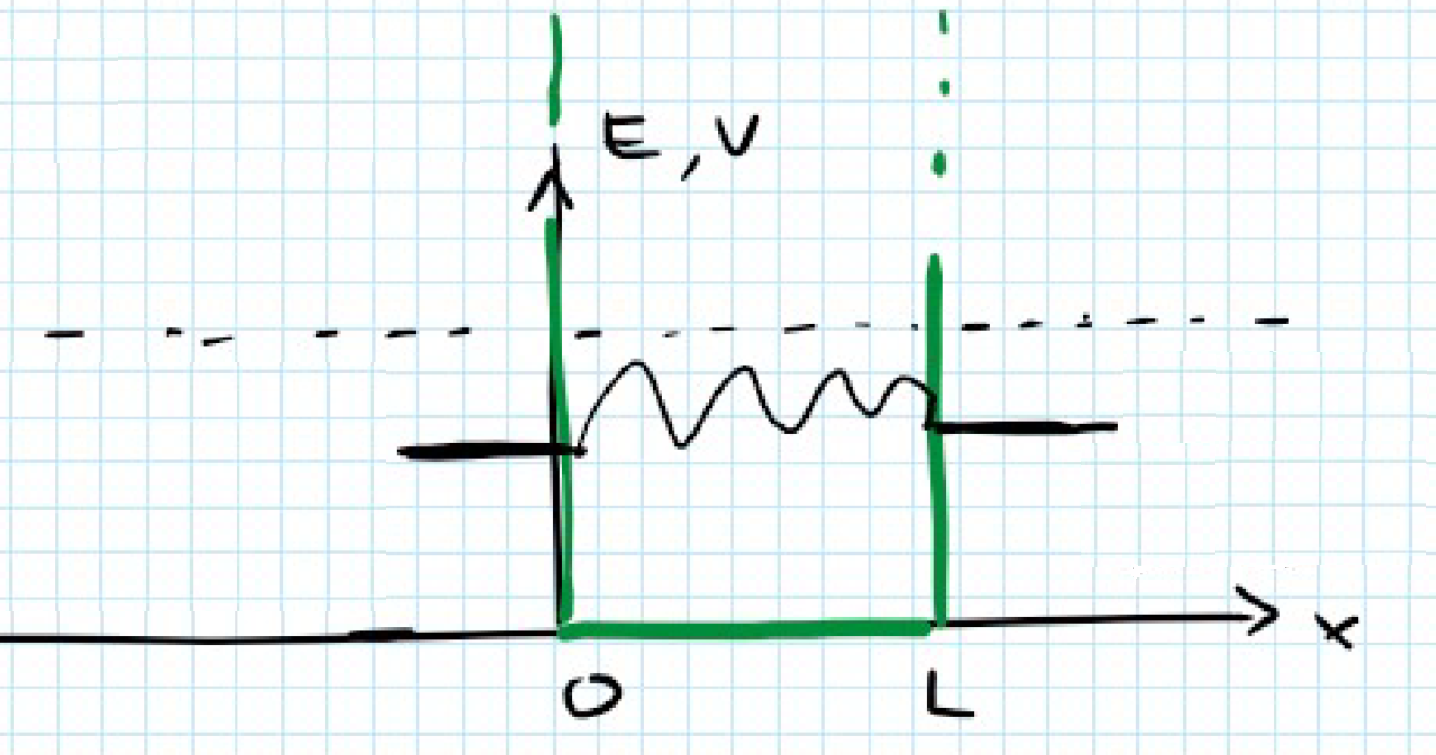
\includegraphics[width=5.4cm]{images/buca_infinita.png}
\end{figure}

\noindent
Se siamo nella regione $x<0$ o $x>L$ allora ogni valore di energia \`e sicuramente minore di $\infty$, quindi non abbiamo soluzione. Se siamo nella regione $0\leq x\leq L$ allora per $E$ positive abbiamo soluzioni della forma
\[\psi(x,t)=\wt Ae^{-i(\omega t-kx)}+\wt Be^{-i(\omega t+kx)}\]
come prima, o passando alla parte indipendente dal tempo
\[f(x)=A\cos(kx)+B\sin(kx).\]
Per avere compatibilit\`a tra le due regioni $\psi(0)=\psi(L)=0$, cio\`e
\[Ae^{-i\omega t}=\psi(0)=0\implies A=0\]
e similmente
\[B\sin(kL)=0\implies k\in \frac \pi L\Z.\]
Quindi le soluzioni sono della forma
\[\psi_n(x,t)=B\sin\pa{\frac{n\pi}L x} e^{-i\omega t}=e^{-i\omega t}f_n(x)\]
al variare di $n\in\Z$. Possiamo ricavare $B$ imponendo la normalizzazione
\begin{align*}
1=&\int_0^L\abs{\psi(x,t)}^2dx=B^2\int_0^L\sin^2\pa{\frac{n\pi}L x}dx=\\
=&B^2\frac{L}{n\pi}\int_0^{n\pi} \sin^2(u)du=\\
=&B^2\frac{L}{n\pi}\frac{n\pi}2=B^2\frac L2,
\end{align*}
da cui $B=\sqrt{2/L}$.

\begin{remark}[Energie possibili]
Non tutti i valori di energia sono possibili, le uniche possibilit\`a sono
\[E=\frac{\hbar^2k^2}{2m}=\frac{\hbar^2n^2\pi^2}{2\pi L^2}.\]
Questo \`e molto strano, perch\'e nel caso classico ci aspetteremmo una distribuzione uniforme.\\
Se per\`o consideriamo il limite $n\to\infty$ allora ritroviamo il caso classico. Poich\'e a $n$ grande corrisponde $E$ grande ha senso ritrovare il caso classico in questa circostanza.

\begin{figure}[!htb]
    \centering
    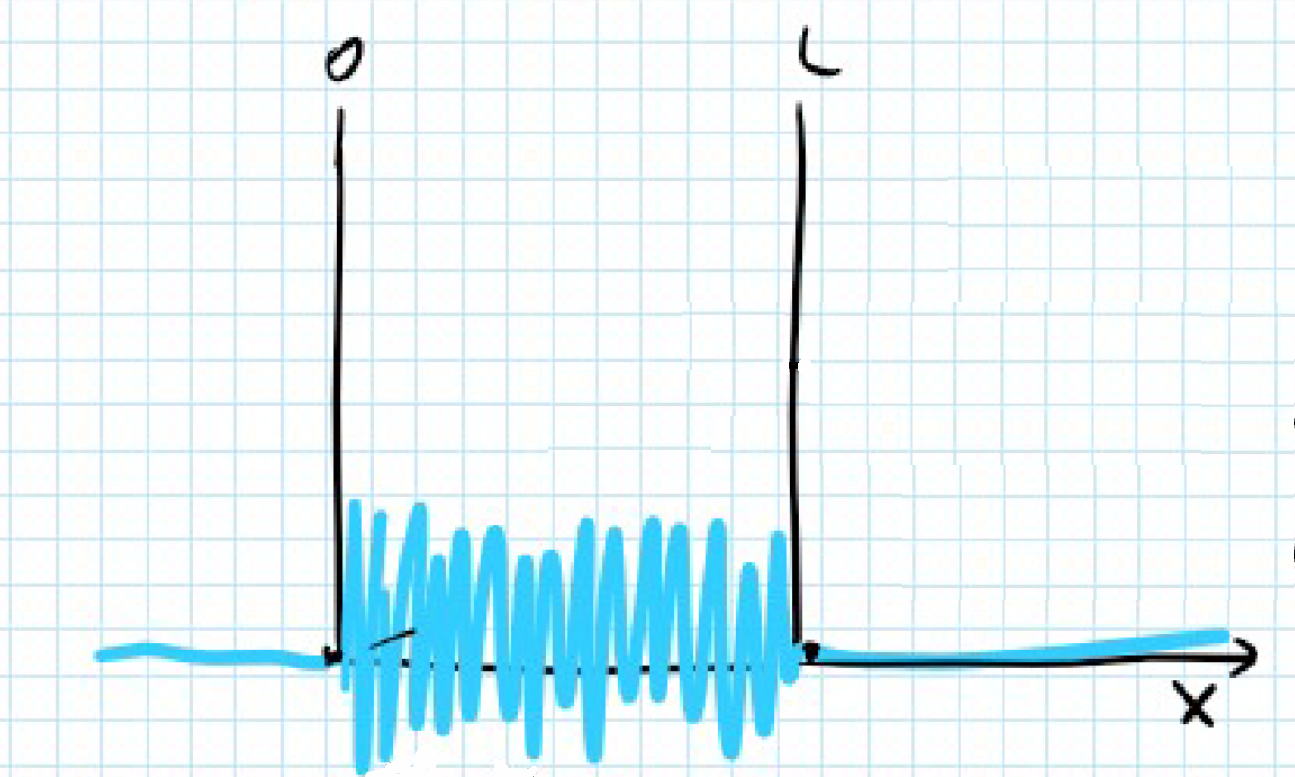
\includegraphics[width=6cm]{images/principio_di_corrispondenza.png}
\end{figure}
\end{remark}

\begin{fact}[Principio di corrispondenza]
Nel limite $n\to\infty$ ritroviamo le soluzioni classiche.
\end{fact}

\begin{fact}
Ogni soluzione all'equazione di Schr\"odinger indipendente dal tempo nella regione $0<x<L$ si pu\`o scrivere come combinazione lineare (potenzialmente infinita) delle $f_n$
\[f(x)=\sum c_n f_n(x),\]
dove $c_n=\int_0^L f_n^\ast(x) f(x)dx$ e $\int_0^L f_n(x)f_m(x)dx=\delta_{nm}$.\bigskip

\noindent Segue che le soluzioni all'equazione di Schr\"odinger in questa regione sono
\[\psi=\sum_n c_n e^{-iE_i t/\hbar} f_n\]
\end{fact}

\begin{example}
Consideriamo $f(x)=c_1f_1(x)+c_2f_2(x)$ dove la prima soluzione ha energia $E_1$ e la seconda $E_2$. Allora
\[\abs{\psi}^2=\abs{c_1}^2 f_1^2+\abs{c_2}^2 f_2^2+2c_1^\ast c_2 f_1f_2 e^{-i(E_2-E_1)t/\hbar}\]
dove il termine $2c_1^\ast c_2 f_1f_2 e^{-i(E_2-E_1)t/\hbar}$ NON \`e indipendente dal tempo, dunque questa $\psi$ NON \`e una soluzione stazionaria, nonostante sia la somma di due stazionarie.
\end{example}



\subsubsection{Potenziale buca finita}
Consideriamo un potenziale del tipo
\[V(x)=\begin{cases}
0 &\abs{x}\leq L\\
V_0 &\abs{x}>L
\end{cases}\]

\begin{figure}[!htb]
    \centering
    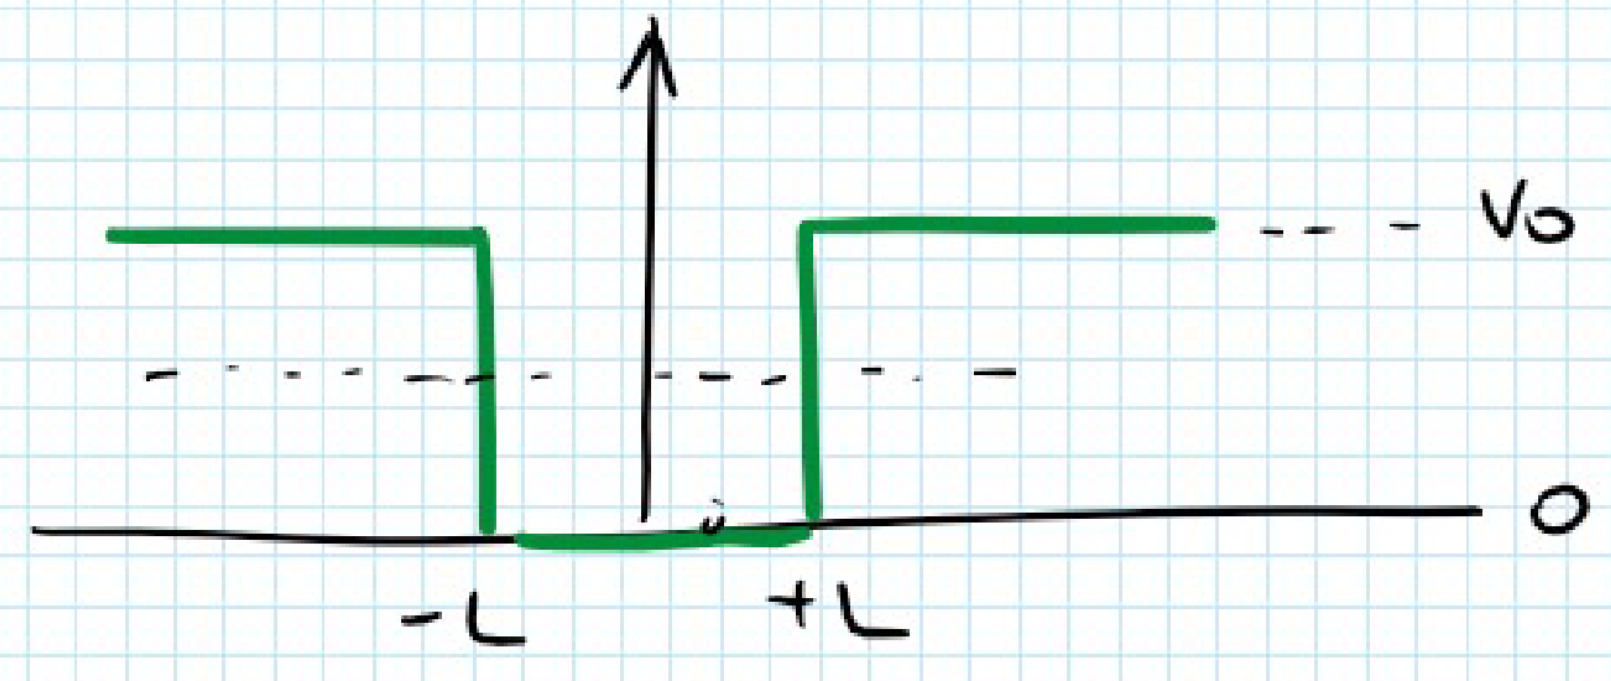
\includegraphics[width=7cm]{images/buca_finita.png}
\end{figure}

\noindent Consideriamo tre casi
\setlength{\leftmargini}{0cm}
\begin{itemize}
\item[$\boxed{E>V_0}$] In questo caso $k$ \`e reale ovunque, quindi eventuali soluzioni non sarebbero normalizzabili.
\item[$\boxed{E<0}$] Non esistono soluzioni non nulle.
\item[$\boxed{0<E<V_0}$] In questo caso le soluzioni assumono la forma
\[f(x)=\begin{cases}
A_1e^{\al x}+B_1 e^{-\al x} & x<-L\\
A_2\sin(kx)+B_2\cos(kx) &\abs x\leq L\\
A_3e^{\al x}+B_3 e^{-\al x} & x>L
\end{cases}\]
dove $\al=\sqrt{\frac{2m(V_0-E)}{\hbar^2}}$ e $k=\sqrt{\frac{2mE}{\hbar^2}}$. Affinch\'e una $f$ cos\`i definita sia valida devono valere le seguenti condizioni:
\begin{itemize}
\item Normalizzazione, cio\`e $\int_{-\infty}^\infty \abs{\psi(x,t)}^2dx=1$,
\item $\displaystyle\lim_{\abs{x}\to+\infty}f(x)=0$,
\item continuit\`a in $\pm L$,
\item continuit\`a\footnote{non avevamo chiesto la continuit\`a della derivata nel caso di buca infinita perch\'e quel problema non \`e realistico.} di $f'$ in $\pm L$.
\end{itemize}
Queste sono $1+2+2+2=7$ condizioni su $7$ parametri (anche $E$ \`e un parametro per $f$ perch\'e appare nella definizione di $\al$ e $k$). La seconda condizione corrisponde semplicemente a $B_1=A_3=0$. Le condizioni di continuit\`a restituiscono la seguente equazione matriciale
\[\mat{
e^{-\al L} & \sin(kL) & -\cos(kL) & 0\\
0 & -\sin(kL) & -\cos(kL) & e^{-\al L}\\
\al e^{-\al L} & k\cos(kL) &-k\sin(kL) &0\\
0 & -k\cos(kL) & -k\sin(kL) &\al e^{-\al L}
}\mat{A_1\\ A_2\\ B_2\\ B_3}=\mat{0\\0\\0\\0},\]
o equivalentemente, facendo diverse operazioni di riga che preservano il nucleo e riordinando le variabili,
\[\mat{
e^{-\al L} &0& \sin(kL) & -\cos(kL) \\
0 & e^{-\al L}& -\sin(kL) & -\cos(kL) \\
0 & 0 & k\cos(kL)-\al \sin(kL) &0 \\
0 & 0 & 0 & -k\sin(kL)+\al \cos(kL)
}\mat{A_1\\ B_3\\ A_2\\ B_2}=\mat{0\\0\\0\\0}.\]
Se $-k\sin(kL)+\al \cos(kL)\neq 0$ allora vediamo che questa matrice ha 4 pivot, quindi l'unico elemento del nucleo \`e il vettore nullo, che restituisce una soluzione banale, quindi abbiamo soluzioni non banali solo se i valori di $E$ per i quali $\al=k\tan(kL)$, che sono finiti. In questo caso $A_2$ e $B_2$ risultano liberi e determinano $A_1$ e $B_3$. Imporre la normalizzazione restituisce una condizione su $A_2$ e $B_2$, che comunque ci lascia un grado di liber\`a.\bigskip

\noindent
Una soluzione generica ha questa forma

\begin{figure}[!htb]
    \centering
    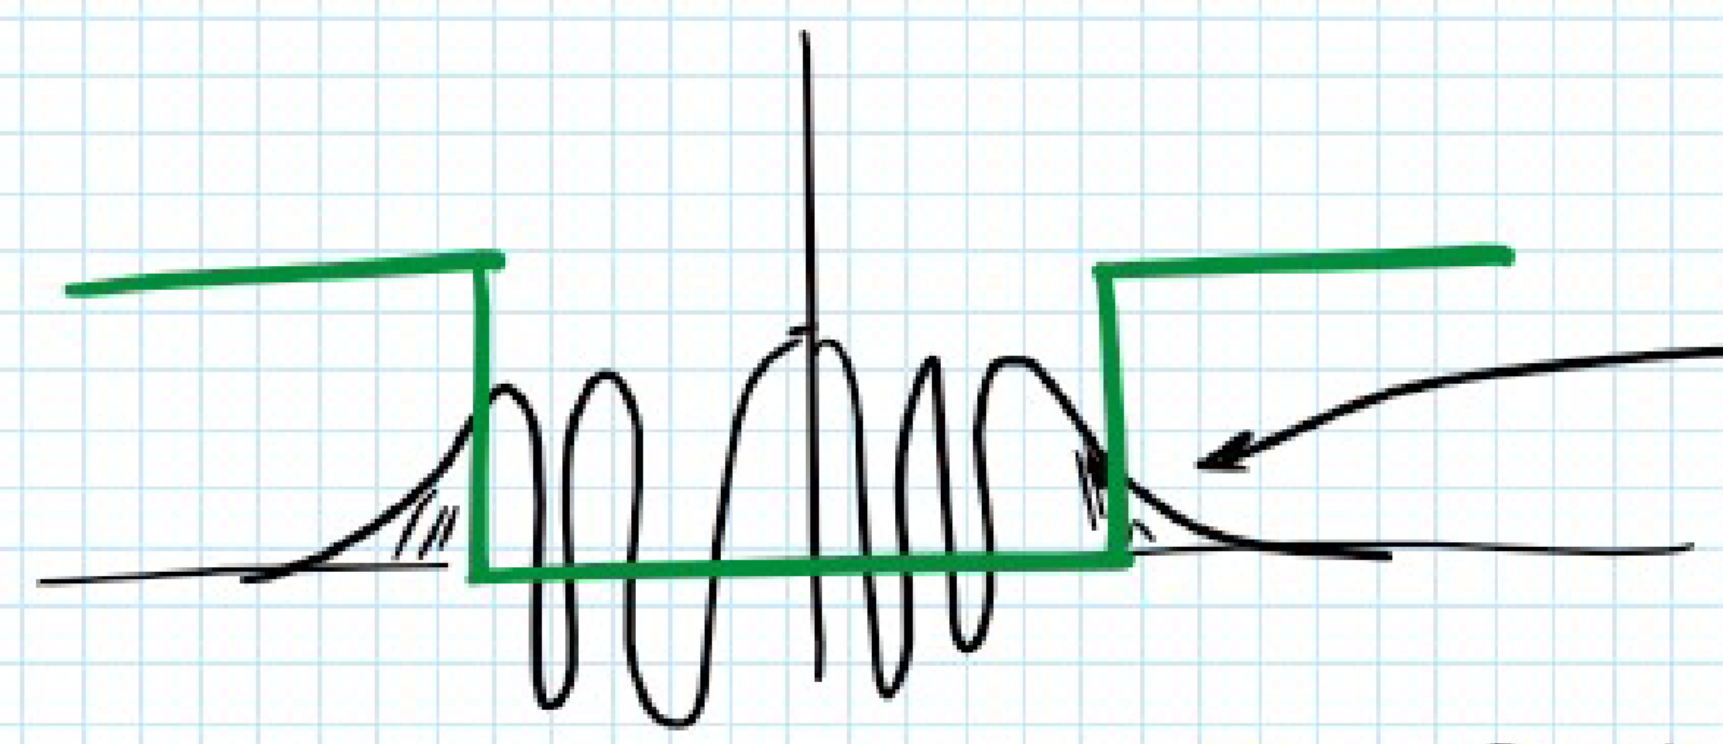
\includegraphics[width=7cm]{images/soluzione_buca_finita.png}
\end{figure}

La densit\`a di probabilit\`a dentro i muri e vicino ai bordi non \`e nulla, quindi \`e possibile che la particella venga misurata DENTRO IL MURO.
\end{itemize}
\setlength{\leftmargini}{0.5cm}


\subsubsection{Potenziale barriera finita}

Consideriamo un potenziale del tipo
\[V(x)=\begin{cases}
V_0 &\abs{x}\leq L\\
0 &\abs{x}>L
\end{cases}\]
\noindent
Risolvendo troviamo anche soluzioni come

\begin{figure}[!htb]
    \centering
    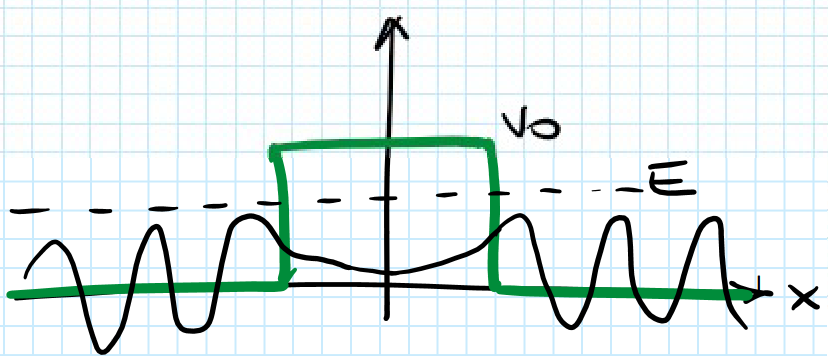
\includegraphics[width=7cm]{images/Barriera_finita.png}
\end{figure}

\noindent
in particolare se piazziamo una particella da un lato del muro e aspettiamo, la funzione d'onda evolve in modo tale che la probabilit\`a di trovarla dall'altra parte del muro diventa non nulla. Questo \`e detto \textbf{effetto tunnel}.

\begin{example}[Fusione nucleare]
In una stessa due nuclei, entrambi con carica positiva dunque, possono collidere e fondersi. Questo fenomeno classicamente non \`e concepibile dato che la forza elettrica diventerebbe abbastanza forte da non farli collidere

\begin{figure}[!htb]
    \centering
    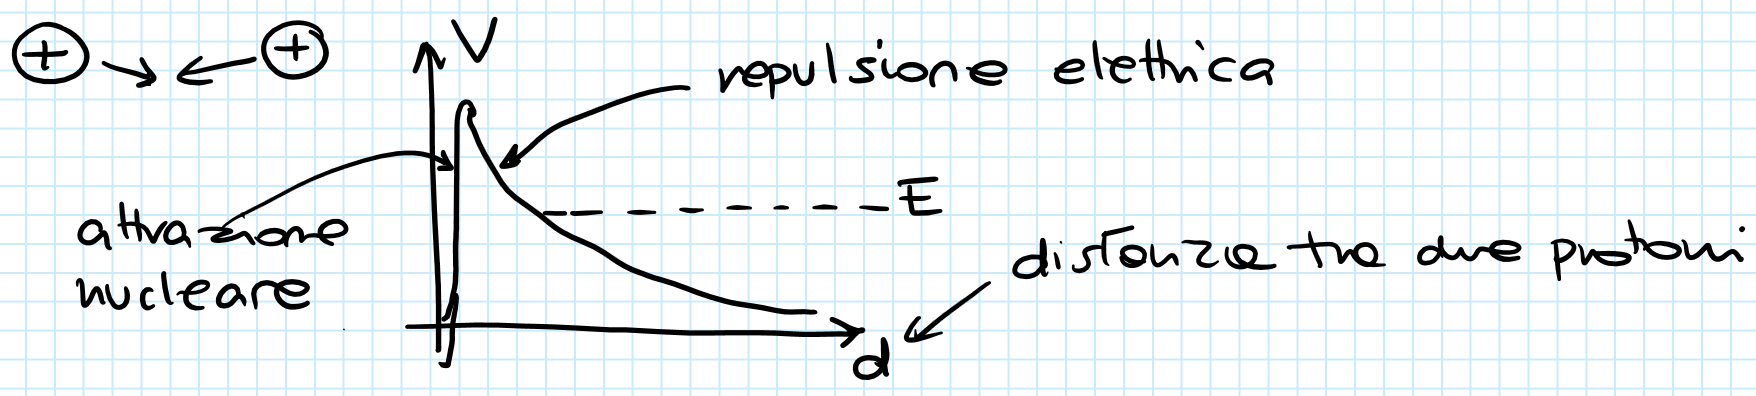
\includegraphics[width=12cm]{images/Fusione_nucleare.png}
\end{figure}

\noindent Considerando per\`o l'effetto tunnel, \`e possibile che i protoni semplicemente superino la barriera del potenziale in quanto c'\`e una probabilit\`a non nulla che lo facciano. In questo senso l'effetto tunnel spiega perch\'e avviene la fusione nucleare, apparentemente impossibile data la differenza tra l'energia media delle particelle coinvolte e il potenziale che dovrebbero superare per realizzare la fusione.
\end{example}
